\documentclass[12pt, a4paper]{ctexart}
\usepackage{geometry}
\geometry{left=2.5cm, right=2.5cm, top=3cm, bottom=3cm}
\usepackage{amsmath}
\usepackage{circuitikz}
\usepackage{subcaption}
\usepackage{float}
\usepackage{tikz-timing}
\usepackage{multirow}
\usetikzlibrary{arrows, shapes.gates.logic.US}
\tikzset{
    dot/.style={circle, fill, inner sep=1pt}
}
\ctikzset{
    logic ports=ieee,
    logic ports/scale=0.8,
    multipoles/flipflop/pin spacing=0.4
}

\begin{document}

\section*{第4章习题}

\subsection*{4.}

忽略逻辑门的传输延迟，画出波形图如下

\begin{figure}[H]
    \centering
    \begin{tikztimingtable}[
        timing/slope=0,
        xscale=3,
        yscale=2
    ]
        $S$ & L 3H 5L 3H 3L \\
        $R$ & 7L 5H 3L\\
        $Q$ & L 6H 5L 3X\\
        $\overline{Q}$ & H 6L 2H 3L 3X\\
        \extracode
        \vertlines[dashed]{0,...,15}
    \end{tikztimingtable}
    \caption{SR锁存器的波形图}
\end{figure}

\subsection*{5.}

忽略逻辑门的传输延迟，画出波形图如下

\begin{figure}[H]
    \centering
    \begin{tikztimingtable}[
        timing/slope=0,
        xscale=2,
        yscale=2
    ]
        $D$ & L H 2L H 2L 6H 4L 2H\\
        $C$ & 3L 3H 3L 3H 3L 3H L\\
        $Q$ & 4L H 4L 6H 2L 2H\\
        $\overline{Q}$ & 4H L 4H 6L 2H 2L\\
    \end{tikztimingtable}
    \caption{D锁存器的波形图}
\end{figure}

\begin{figure}[H]
    \centering
    \begin{tikztimingtable}[
        timing/slope=0,
        xscale=2,
        yscale=2
    ]
        $D$ & L H 2L H 2L 6H 4L 2H\\
        $Clk$ & 3L 3H 3L 3H 3L 3H L\\
        $Q$ & 9L 6H 4L\\
        $\overline{Q}$ & 9H 6L 4H\\
    \end{tikztimingtable}
    \caption{D触发器的波形图}
\end{figure}

\subsection*{6.}

由 $En=D\oplus Q$ 可画出构造的电路图

\begin{figure}[H]
    \centering
    \begin{circuitikz}
        \node [
            flipflop T,
            flipflop def={t1=En,t3=T}
        ] (T) at (0,0) {};
        \node[xor gate US, draw] (xor) at (-2,0 |- T.pin 1) {};
        \draw (T.pin 1) -- (xor.output);
        \draw (xor.input 1) -| (-3,1.5) -- (2,1.5) |- node[dot]{} (T.pin 6);
        \draw (xor.input 2) -- (-4,0 |- xor.input 2) node[left] (D) {$D$};
        \draw (T.pin 3) -- (-4,0 |- T.pin 3) node[left] {$Clk$};
        \draw (T.pin 6) --++ (2,0) node[right] (Q) {$Q$};
        \draw (T.pin 4) --++ (2,0) node[right] (nQ) {$\overline{Q}$};
        \draw[dashed] (-3.5,2) -- (-3.5,-1.5) -- (2.5,-1.5) -- (2.5,2) -- (-3.5,2);
    \end{circuitikz}
    \caption{用T触发器构造的D触发器}
\end{figure}

\subsection*{9.}

本题有三个状态，需要 $\lceil\log_23\rceil=2$ 个D触发器，可得状态表如下

\begin{table}[H]
    \centering
    \begin{tabular}{|c|cc|}
    \hline
    \multirow{2}{*}{$Y_1Y_0$} & \multicolumn{2}{c|}{$Y^*/Z$} \\ \cline{2-3} 
         & \multicolumn{1}{c|}{$X=0$}    & $X=1$    \\ \hline
    $00$ & \multicolumn{1}{c|}{$00/Z=0$} & $01/Z=0$ \\ \hline
    $01$ & \multicolumn{1}{c|}{$00/Z=0$} & $10/Z=0$ \\ \hline
    $10$ & \multicolumn{1}{c|}{$00/Z=1$} & $10/Z=0$ \\ \hline
    \end{tabular}
    \caption{110序列检测状态表}
\end{table}

若希望电路状态为11时，可在一个时钟周期后回到初始状态00，可计算出次态逻辑函数与输出逻辑函数

\begin{equation}
    Y_0^*=X\overline Y_0\overline Y_1,
    Y_1^*=X(Y_0\oplus Y_1),
    Z=\overline X\,\overline Y_0Y_1
\end{equation}

据此设计电路图如下

\begin{figure}[H]
    \centering
    \begin{circuitikz}
        \node[not gate US, draw] (not0) at (3.5,1.5) {};
        \draw (-4,1.5) node[left] (X) {$X$} -- (not0.input);
        \draw (not0.output) -- (5,1.5);
        \node[flipflop D, flipflop def={t3=C}] (D0) at (0,0) {$D_0$};
        \node[flipflop D, flipflop def={t3=C}] (D1) at (0,-2) {$D_1$};
        \draw (D0.pin 6) -- (5,0 |- D0.pin 6);
        \draw (D0.pin 4) -- (5,0 |- D0.pin 4);
        \draw (D1.pin 6) -- (5,0 |- D1.pin 6);
        \draw (D1.pin 4) -- (5,0 |- D1.pin 4);
        \node[and port, number inputs=3, rotate=-90] (and0) at (1.5,-4) {};
        \node[xor port, rotate=-90] (xor) at (3,-4) {};
        \node[and port, number inputs=3, rotate=-90] (and1) at (4.5,-4) {};
        \draw (X) -| node[dot]{} (and0.in 3);
        \draw (D0.pin 4) -| node[dot]{} (and0.in 2);
        \draw (D1.pin 4) -| node[dot]{} (and0.in 1);
        \draw (D0.pin 6) -| node[dot]{} (xor.in 2);
        \draw (D1.pin 6) -| node[dot]{} (xor.in 1);
        \draw (not0.output) -| node[dot]{} (and1.in 3);
        \draw (D0.pin 4) -| node[dot]{} (and1.in 2);
        \draw (D1.pin 6) -| node[dot]{} (and1.in 1);
        \node[and port, rotate=90] (and2) at (-2.5,-4) {};
        \draw (and0.out) -| (-1.5,-4) |- (D0.pin 1);
        \draw (xor.out) -- (3,-5.2) -| (and2.in 2);
        \draw (X) -| node[dot]{} (-3.5,-5.2) -| (and2.in 1);
        \draw (and2.out) |- (D1.pin 1);
        \node[below] at (and1.out) (Z) {$Z$};
        \draw (D1.pin 3) -- (-4,0 |- D1.pin 3) node[left] (Clk) {$Clk$};
        \draw (D0.pin 3) -| (-3,0 |- D1.pin 3) node[dot]{};
    \end{circuitikz}
    \caption{110序列检测电路图（2个D触发器）}
\end{figure}

如果触发器数目没有限制，可以简化逻辑，让 $Z=\overline{Q_0}Q_1Q_2$，画出电路图如下

\begin{figure}[H]
    \centering
    \begin{circuitikz}
        \node[flipflop D, flipflop def={t3=C}] (D0) at (0,0) {$D_0$};
        \node[flipflop D, flipflop def={t3=C}] (D1) at (3,0) {$D_1$};
        \node[flipflop D, flipflop def={t3=C}] (D2) at (6,0) {$D_2$};
        \draw (D0.pin 6) -- (D1.pin 1);
        \draw (D1.pin 6) -- (D2.pin 1);
        \node[left] at (-2,0 |- D0.pin 1) (X) {$X$};
        \node[left] at (-2,-1.2) (Clk) {$Clk$};
        \draw (X) -- (D0.pin 1);
        \draw (Clk) -| node[dot]{} (D0.pin 3);
        \draw (Clk) -| node[dot]{} (D1.pin 3);
        \draw (Clk) -| (D2.pin 3);
        \node[and port, number inputs=3] (and) at (8,1.2) {};
        \node[right] at (and.out) (Z) {$Z$};
        \draw (D0.pin 4) |- (and.in 1);
        \draw (D1.pin 6) node[dot]{} |- (and.in 2);
        \draw (D2.pin 6) |- (and.in 3);
    \end{circuitikz}
    \caption{110序列检测电路图（3个D触发器）}
\end{figure}

\subsection*{11.}

由于时钟周期 $t_{\text{clk}}$ 满足

\begin{equation}
    t_{\text{clk}}>t_{\text{ffpd}}+t_{\text{nspd}}+t_{\text{setup}}
    =T_{\text{tq}}+T_{\text{and}}+T_{\text{setup}}
\end{equation}

所以 Clk 的最大工作频率为 $\dfrac1{t_{\text{clk}}}=\dfrac1{T_{\text{tq}}+T_{\text{and}}+T_{\text{setup}}}$

\subsection*{12.}

$Q_3Q_2Q_1Q_0$ 的编码转换情况为

\begin{table}[H]
    \centering
    \begin{tabular}{|cc|cc|cc|cc|}
        \hline
        $Q$  & $Q^*$ & $Q$  & $Q^*$ & $Q$  & $Q^*$ & $Q$  & $Q^*$ \\ \hline
        0000 & 0000  & 0100 & 1010  & 1000 & 1100  & 1100 & 0110  \\ \hline
        0001 & 0000  & 0101 & 1010  & 1001 & 1100  & 1101 & 0110  \\ \hline
        0010 & 0001  & 0110 & 1011  & 1010 & 1101  & 1110 & 0111  \\ \hline
        0011 & 0001  & 0111 & 1011  & 1011 & 1101  & 1111 & 0111  \\ \hline
    \end{tabular}
    \caption{编码转换表}
\end{table}

根据表格，可画出状态转移图

\begin{figure}[H]
    \centering
    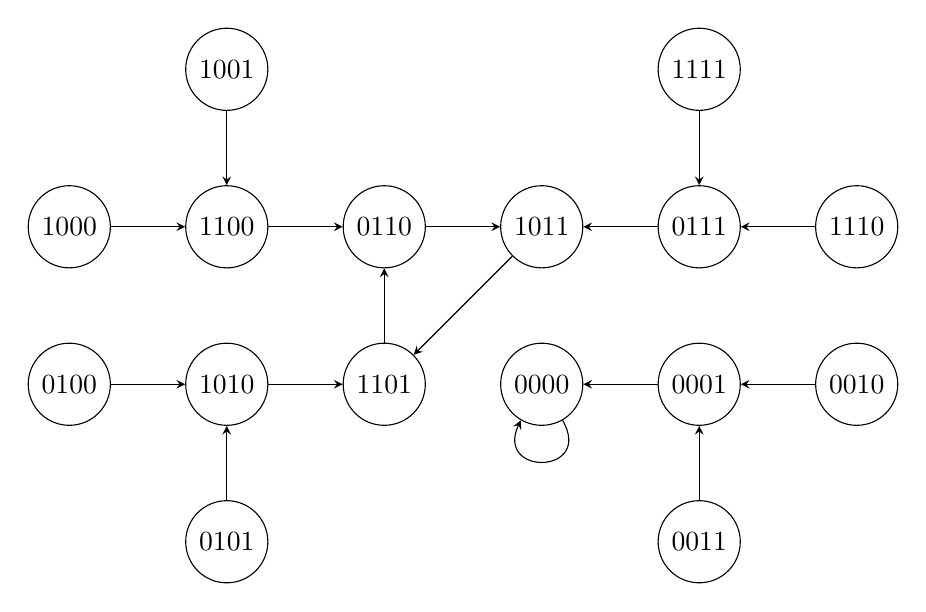
\begin{tikzpicture}[>=stealth]
        \node[circle, draw] (0110) at (0,0) {0110};
        \node[circle, draw] (1011) at (2,0) {1011};
        \node[circle, draw] (1101) at (0,-2) {1101};
        \node[circle, draw] (0000) at (2,-2) {0000};
        \draw[->] (0110) -- (1011);
        \draw[->] (1011) -- (1101);
        \draw[->] (1101) -- (0110);
        \node[circle, draw] (1100) at (-2,0) {1100};
        \node[circle, draw] (1010) at (-2,-2) {1010};
        \node[circle, draw] (0111) at (4,0) {0111};
        \node[circle, draw] (0001) at (4,-2) {0001};
        \draw[->] (1100) -- (0110);
        \draw[->] (1010) -- (1101);
        \draw[->] (0111) -- (1011);
        \draw[->] (0001) -- (0000);
        \node[circle, draw] (1000) at (-4,0) {1000};
        \node[circle, draw] (1001) at (-2,2) {1001};
        \draw[->] (1000) -- (1100);
        \draw[->] (1001) -- (1100);
        \node[circle, draw] (0100) at (-4,-2) {0100};
        \node[circle, draw] (0101) at (-2,-4) {0101};
        \draw[->] (0100) -- (1010);
        \draw[->] (0101) -- (1010);
        \node[circle, draw] (1110) at (6,0) {1110};
        \node[circle, draw] (1111) at (4,2) {1111};
        \draw[->] (1110) -- (0111);
        \draw[->] (1111) -- (0111);
        \node[circle, draw] (0010) at (6,-2) {0010};
        \node[circle, draw] (0011) at (4,-4) {0011};
        \draw[->] (0010) -- (0001);
        \draw[->] (0011) -- (0001);
        \draw[->] (0000) edge [out=300, in=240, loop, looseness=4] (0000);
    \end{tikzpicture}
    \caption{状态转移图}
\end{figure}

可见，图中有一个长度为3的环和一个长度为1的环，其他状态经过有限次转移后都能进入这两个环。

\end{document}